\PassOptionsToPackage{unicode=true}{hyperref} % options for packages loaded elsewhere
\PassOptionsToPackage{hyphens}{url}
%
\documentclass[]{article}
\usepackage{lmodern}
\usepackage{amssymb,amsmath}
\usepackage{ifxetex,ifluatex}
\usepackage{fixltx2e} % provides \textsubscript
\ifnum 0\ifxetex 1\fi\ifluatex 1\fi=0 % if pdftex
  \usepackage[T1]{fontenc}
  \usepackage[utf8]{inputenc}
  \usepackage{textcomp} % provides euro and other symbols
\else % if luatex or xelatex
  \usepackage{unicode-math}
  \defaultfontfeatures{Ligatures=TeX,Scale=MatchLowercase}
\fi
% use upquote if available, for straight quotes in verbatim environments
\IfFileExists{upquote.sty}{\usepackage{upquote}}{}
% use microtype if available
\IfFileExists{microtype.sty}{%
\usepackage[]{microtype}
\UseMicrotypeSet[protrusion]{basicmath} % disable protrusion for tt fonts
}{}
\IfFileExists{parskip.sty}{%
\usepackage{parskip}
}{% else
\setlength{\parindent}{0pt}
\setlength{\parskip}{6pt plus 2pt minus 1pt}
}
\usepackage{hyperref}
\hypersetup{
            pdftitle={Adult Income Study: Milestone 03},
            pdfauthor={Jimmy Liu and Hannah McSorley},
            pdfborder={0 0 0},
            breaklinks=true}
\urlstyle{same}  % don't use monospace font for urls
\usepackage[margin=1in]{geometry}
\usepackage{color}
\usepackage{fancyvrb}
\newcommand{\VerbBar}{|}
\newcommand{\VERB}{\Verb[commandchars=\\\{\}]}
\DefineVerbatimEnvironment{Highlighting}{Verbatim}{commandchars=\\\{\}}
% Add ',fontsize=\small' for more characters per line
\usepackage{framed}
\definecolor{shadecolor}{RGB}{248,248,248}
\newenvironment{Shaded}{\begin{snugshade}}{\end{snugshade}}
\newcommand{\AlertTok}[1]{\textcolor[rgb]{0.94,0.16,0.16}{#1}}
\newcommand{\AnnotationTok}[1]{\textcolor[rgb]{0.56,0.35,0.01}{\textbf{\textit{#1}}}}
\newcommand{\AttributeTok}[1]{\textcolor[rgb]{0.77,0.63,0.00}{#1}}
\newcommand{\BaseNTok}[1]{\textcolor[rgb]{0.00,0.00,0.81}{#1}}
\newcommand{\BuiltInTok}[1]{#1}
\newcommand{\CharTok}[1]{\textcolor[rgb]{0.31,0.60,0.02}{#1}}
\newcommand{\CommentTok}[1]{\textcolor[rgb]{0.56,0.35,0.01}{\textit{#1}}}
\newcommand{\CommentVarTok}[1]{\textcolor[rgb]{0.56,0.35,0.01}{\textbf{\textit{#1}}}}
\newcommand{\ConstantTok}[1]{\textcolor[rgb]{0.00,0.00,0.00}{#1}}
\newcommand{\ControlFlowTok}[1]{\textcolor[rgb]{0.13,0.29,0.53}{\textbf{#1}}}
\newcommand{\DataTypeTok}[1]{\textcolor[rgb]{0.13,0.29,0.53}{#1}}
\newcommand{\DecValTok}[1]{\textcolor[rgb]{0.00,0.00,0.81}{#1}}
\newcommand{\DocumentationTok}[1]{\textcolor[rgb]{0.56,0.35,0.01}{\textbf{\textit{#1}}}}
\newcommand{\ErrorTok}[1]{\textcolor[rgb]{0.64,0.00,0.00}{\textbf{#1}}}
\newcommand{\ExtensionTok}[1]{#1}
\newcommand{\FloatTok}[1]{\textcolor[rgb]{0.00,0.00,0.81}{#1}}
\newcommand{\FunctionTok}[1]{\textcolor[rgb]{0.00,0.00,0.00}{#1}}
\newcommand{\ImportTok}[1]{#1}
\newcommand{\InformationTok}[1]{\textcolor[rgb]{0.56,0.35,0.01}{\textbf{\textit{#1}}}}
\newcommand{\KeywordTok}[1]{\textcolor[rgb]{0.13,0.29,0.53}{\textbf{#1}}}
\newcommand{\NormalTok}[1]{#1}
\newcommand{\OperatorTok}[1]{\textcolor[rgb]{0.81,0.36,0.00}{\textbf{#1}}}
\newcommand{\OtherTok}[1]{\textcolor[rgb]{0.56,0.35,0.01}{#1}}
\newcommand{\PreprocessorTok}[1]{\textcolor[rgb]{0.56,0.35,0.01}{\textit{#1}}}
\newcommand{\RegionMarkerTok}[1]{#1}
\newcommand{\SpecialCharTok}[1]{\textcolor[rgb]{0.00,0.00,0.00}{#1}}
\newcommand{\SpecialStringTok}[1]{\textcolor[rgb]{0.31,0.60,0.02}{#1}}
\newcommand{\StringTok}[1]{\textcolor[rgb]{0.31,0.60,0.02}{#1}}
\newcommand{\VariableTok}[1]{\textcolor[rgb]{0.00,0.00,0.00}{#1}}
\newcommand{\VerbatimStringTok}[1]{\textcolor[rgb]{0.31,0.60,0.02}{#1}}
\newcommand{\WarningTok}[1]{\textcolor[rgb]{0.56,0.35,0.01}{\textbf{\textit{#1}}}}
\usepackage{graphicx,grffile}
\makeatletter
\def\maxwidth{\ifdim\Gin@nat@width>\linewidth\linewidth\else\Gin@nat@width\fi}
\def\maxheight{\ifdim\Gin@nat@height>\textheight\textheight\else\Gin@nat@height\fi}
\makeatother
% Scale images if necessary, so that they will not overflow the page
% margins by default, and it is still possible to overwrite the defaults
% using explicit options in \includegraphics[width, height, ...]{}
\setkeys{Gin}{width=\maxwidth,height=\maxheight,keepaspectratio}
\setlength{\emergencystretch}{3em}  % prevent overfull lines
\providecommand{\tightlist}{%
  \setlength{\itemsep}{0pt}\setlength{\parskip}{0pt}}
\setcounter{secnumdepth}{0}
% Redefines (sub)paragraphs to behave more like sections
\ifx\paragraph\undefined\else
\let\oldparagraph\paragraph
\renewcommand{\paragraph}[1]{\oldparagraph{#1}\mbox{}}
\fi
\ifx\subparagraph\undefined\else
\let\oldsubparagraph\subparagraph
\renewcommand{\subparagraph}[1]{\oldsubparagraph{#1}\mbox{}}
\fi

% set default figure placement to htbp
\makeatletter
\def\fps@figure{htbp}
\makeatother


\title{Adult Income Study: Milestone 03}
\author{Jimmy Liu and Hannah McSorley}
\date{2020-03-17}

\begin{document}
\maketitle

\hypertarget{introduction}{%
\subsection{Introduction}\label{introduction}}

The economic well-being of individuals is reliant on their income, where
income is defined as the money an individual (or household) receives on
a regular basis. In the United States, the Census Bureau uses income
(money received before expenses and deductions) to gauge the
population's range of poverty, wealth, and financial security (United
States Census Bureau, 2016). There are a variety of factors that can
influence one's income, including socioeconomic drivers, education and
vocation. This project examines some of the variables that are often
related to income.

\hypertarget{description-of-dataset}{%
\subsection{Description of Dataset}\label{description-of-dataset}}

This project works with a dataset of adult incomes obtained from the
University of California Irvine (UCI)
\href{https://archive.ics.uci.edu/ml/datasets/adult}{Machine Learning
Repository}. The data was donated by Ronny Kohavi and Barry Becker
(Silicon Graphics) and was originally extracted by Barry Becker from the
1994 Census database and used for machine learning predictions of
whether a person makes over \$50,000 per year based on personal factors.

This 1994 income census dataset consists of multivariate categorical and
integer data that describe socioeconomic and personal classifiers of
adults across the USA. Each instance (32,561) is an individual whose
annual income was grouped as either above or below \$50,000. Table 1
shows an overview of the 15 attributes (variables), including whether
each is categorical or integer and a brief interpretation of the
variable.

\includegraphics{FinalReport_milestone03_files/figure-latex/variable-table-1.pdf}

\hypertarget{notes-on-original-dataset}{%
\subsubsection{Notes on original
dataset}\label{notes-on-original-dataset}}

A couple of assumptions were made about these data based on information
on the Census website. It was assumed that ``capital gains'' indicate
non-cash financial benefits (e.g., food stamps, health benefits,
subsidized housing or transportation, employer contributions to
retirement programs, medical and educational expenses, etc.), and that
``capital losses'' include non-cash expenses (such as depreciated value
of assets). We also assumed that ``education number'' indicated the
number of years allotted to education.

It is of note that these data are from 1994 census, and the income
threshold of \$50,000 held a different meaning for wealth than it holds
today. Additionally, as this dataset includes socioeconomic attributes,
it's worth noting that the majority of data instances were dominated by
middle-age, white, US-born, male, private-sector employees. Overall,
there appeared to be a fairly even distribution of individuals across
occupational sectors and the majority of individuals work approximately
40 hours per week.

\hypertarget{project-objectives}{%
\subsection{Project Objectives}\label{project-objectives}}

This project developed data analysis skills in R and R studio with a
strong focus on writing Rscripts and executing script commands via
RStudio Terminal or the command line. The ultimate goal was to generate
a full report using a pipeline of scripts, run in sequence, and to
create a report using `Make'.

\hypertarget{eda-research-questions}{%
\subsubsection{EDA Research Questions}\label{eda-research-questions}}

In this study, we explored the relationships between personal attributes
and quantitative income-related variables with the goal of identifying
relationships and interesting patterns. We focused on addressing the
following exploratory research questions:

\begin{enumerate}
\def\labelenumi{\arabic{enumi}.}
\tightlist
\item
  Is there an observable relationship between personal attributes data
  and income level?
\item
  Does the number of hours worked per week relate more to occupation,
  sex, race, age (or is there no clear relationship)?
\item
  What is the relationship between education and hours worked per week
  (e.g.~does a person work fewer hours if they have completed more
  schooling)?
\end{enumerate}

\hypertarget{plan-of-action}{%
\subsubsection{Plan of Action}\label{plan-of-action}}

The variables that effect income may be confounding and are unlikely to
be direct, therefore these data may not be appropriate for linear
regression analyses. We focus on exploring the relationships variables
and identifying relationships and patterns through the initial project's
exploratory data analysis and first steps of running a data analysis
pipeline.

\hypertarget{exploratory-data-analysis}{%
\subsection{Exploratory Data Analysis}\label{exploratory-data-analysis}}

The original data set was loaded into RStudio where we ran a summary and
performed initial exploratory data analysis. A key discovery was that
the variable `income' was not (as might be expected) annual income
values for each data instance, it was instead a categorical variable
that distinguished whether that instance (row value, person) had earned
more than or less than \$50,000 USD. Below is a summary of the initial
dataset.

\begin{verbatim}
##       age                    workclass         fnlwgt       
##  Min.   :17.00    Private         :22696   Min.   :  12285  
##  1st Qu.:28.00    Self-emp-not-inc: 2541   1st Qu.: 117827  
##  Median :37.00    Local-gov       : 2093   Median : 178356  
##  Mean   :38.58    ?               : 1836   Mean   : 189778  
##  3rd Qu.:48.00    State-gov       : 1298   3rd Qu.: 237051  
##  Max.   :90.00    Self-emp-inc    : 1116   Max.   :1484705  
##                  (Other)          :  981                    
##          education     education.num                  martial_status 
##   HS-grad     :10501   Min.   : 1.00    Divorced             : 4443  
##   Some-college: 7291   1st Qu.: 9.00    Married-AF-spouse    :   23  
##   Bachelors   : 5355   Median :10.00    Married-civ-spouse   :14976  
##   Masters     : 1723   Mean   :10.08    Married-spouse-absent:  418  
##   Assoc-voc   : 1382   3rd Qu.:12.00    Never-married        :10683  
##   11th        : 1175   Max.   :16.00    Separated            : 1025  
##  (Other)      : 5134                    Widowed              :  993  
##             occupation            relationship                    race      
##   Prof-specialty :4140    Husband       :13193    Amer-Indian-Eskimo:  311  
##   Craft-repair   :4099    Not-in-family : 8305    Asian-Pac-Islander: 1039  
##   Exec-managerial:4066    Other-relative:  981    Black             : 3124  
##   Adm-clerical   :3770    Own-child     : 5068    Other             :  271  
##   Sales          :3650    Unmarried     : 3446    White             :27816  
##   Other-service  :3295    Wife          : 1568                              
##  (Other)         :9541                                                      
##       sex         capital.gain    capital.loss    hours.per.week 
##   Female:10771   Min.   :    0   Min.   :   0.0   Min.   : 1.00  
##   Male  :21790   1st Qu.:    0   1st Qu.:   0.0   1st Qu.:40.00  
##                  Median :    0   Median :   0.0   Median :40.00  
##                  Mean   : 1078   Mean   :  87.3   Mean   :40.44  
##                  3rd Qu.:    0   3rd Qu.:   0.0   3rd Qu.:45.00  
##                  Max.   :99999   Max.   :4356.0   Max.   :99.00  
##                                                                  
##         native.country     label      
##   United-States:29170    <=50K:24720  
##   Mexico       :  643    >50K : 7841  
##   ?            :  583                 
##   Philippines  :  198                 
##   Germany      :  137                 
##   Canada       :  121                 
##  (Other)       : 1709
\end{verbatim}

\hypertarget{data-handling}{%
\subsubsection{Data handling}\label{data-handling}}

Summary of the original data showed that `capital-gains' and
`capital-losses' were not categorical values like the `income' variable,
and while these variables were numeric, there were many `zero' values
for capital gains and losses. Because the `income' variable in this
dataset was a binary category (above or below \$50K) the capital gains
and losses appeared to be a more interesting metric in gauging wealth
for the individuals in the Census. Therefore, we filtered the dataset to
include only instances when there was a non-zero value for capital gains
or losses, then combined values of gains and losses to create a `net'
capital gain variable.

To create a data analysis pipeline, data filtering was performed with
Rscripts executed via command line arguments in the RStudio Terminal.
The resulting filtered dataframe (augmented by filtering for instances
that included capital gains and losses) the data demographics were
shifted to slightly older individuals represented by more men than
women. Below is a summary of the filtered dataframe.

\begin{verbatim}
##       age                   workclass        fnlwgt               education   
##  Min.   :17.00   Private         :2714   Min.   :  19302   HS-grad     :1086  
##  1st Qu.:34.00   Self-emp-not-inc: 413   1st Qu.: 118346   Bachelors   : 971  
##  Median :42.00   Local-gov       : 321   Median : 175669   Some-college: 758  
##  Mean   :43.18   Self-emp-inc    : 284   Mean   : 187152   Masters     : 423  
##  3rd Qu.:51.00   ?               : 181   3rd Qu.: 234292   Prof-school : 213  
##  Max.   :90.00   State-gov       : 164   Max.   :1033222   Assoc-voc   : 188  
##                  (Other)         : 154                     (Other)     : 592  
##  education_num                 martial_status             occupation 
##  Min.   : 1.00   Divorced             : 453   Prof-specialty   :850  
##  1st Qu.: 9.00   Married-AF-spouse    :   2   Exec-managerial  :847  
##  Median :10.00   Married-civ-spouse   :2777   Sales            :512  
##  Mean   :11.03   Married-spouse-absent:  35   Craft-repair     :506  
##  3rd Qu.:13.00   Never-married        : 769   Adm-clerical     :362  
##  Max.   :16.00   Separated            :  81   Machine-op-inspct:196  
##                  Widowed              : 114   (Other)          :958  
##          relationship                  race          sex        capital_gain  
##  Husband       :2454   Amer-Indian-Eskimo:  31   Female: 992   Min.   :    0  
##  Not-in-family : 878   Asian-Pac-Islander: 137   Male  :3239   1st Qu.:    0  
##  Other-relative:  71   Black             : 285                 Median : 3137  
##  Own-child     : 258   Other             :  23                 Mean   : 8293  
##  Unmarried     : 274   White             :3755                 3rd Qu.: 7688  
##  Wife          : 296                                           Max.   :99999  
##                                                                               
##   capital_loss    hours_per_week        native_country   label     
##  Min.   :   0.0   Min.   : 1.00   United-States:3850   <=50K:1781  
##  1st Qu.:   0.0   1st Qu.:40.00   ?            :  90   >50K :2450  
##  Median :   0.0   Median :40.00   Mexico       :  31               
##  Mean   : 671.9   Mean   :43.42   Philippines  :  24               
##  3rd Qu.:1740.0   3rd Qu.:50.00   India        :  21               
##  Max.   :4356.0   Max.   :99.00   Germany      :  20               
##                                   (Other)      : 195               
##       net       
##  Min.   :-4356  
##  1st Qu.:-1740  
##  Median : 3137  
##  Mean   : 7622  
##  3rd Qu.: 7688  
##  Max.   :99999  
## 
\end{verbatim}

\hypertarget{eda-relationship-between-education-attainment-and-annual-net-gain}{%
\subsubsection{EDA: Relationship between education attainment and annual
net
gain}\label{eda-relationship-between-education-attainment-and-annual-net-gain}}

As part of exploratory data analysis, we visualized some relationships
among the data. Here we are visualizing the annual net gain across
education levels.

\begin{figure}

{\centering 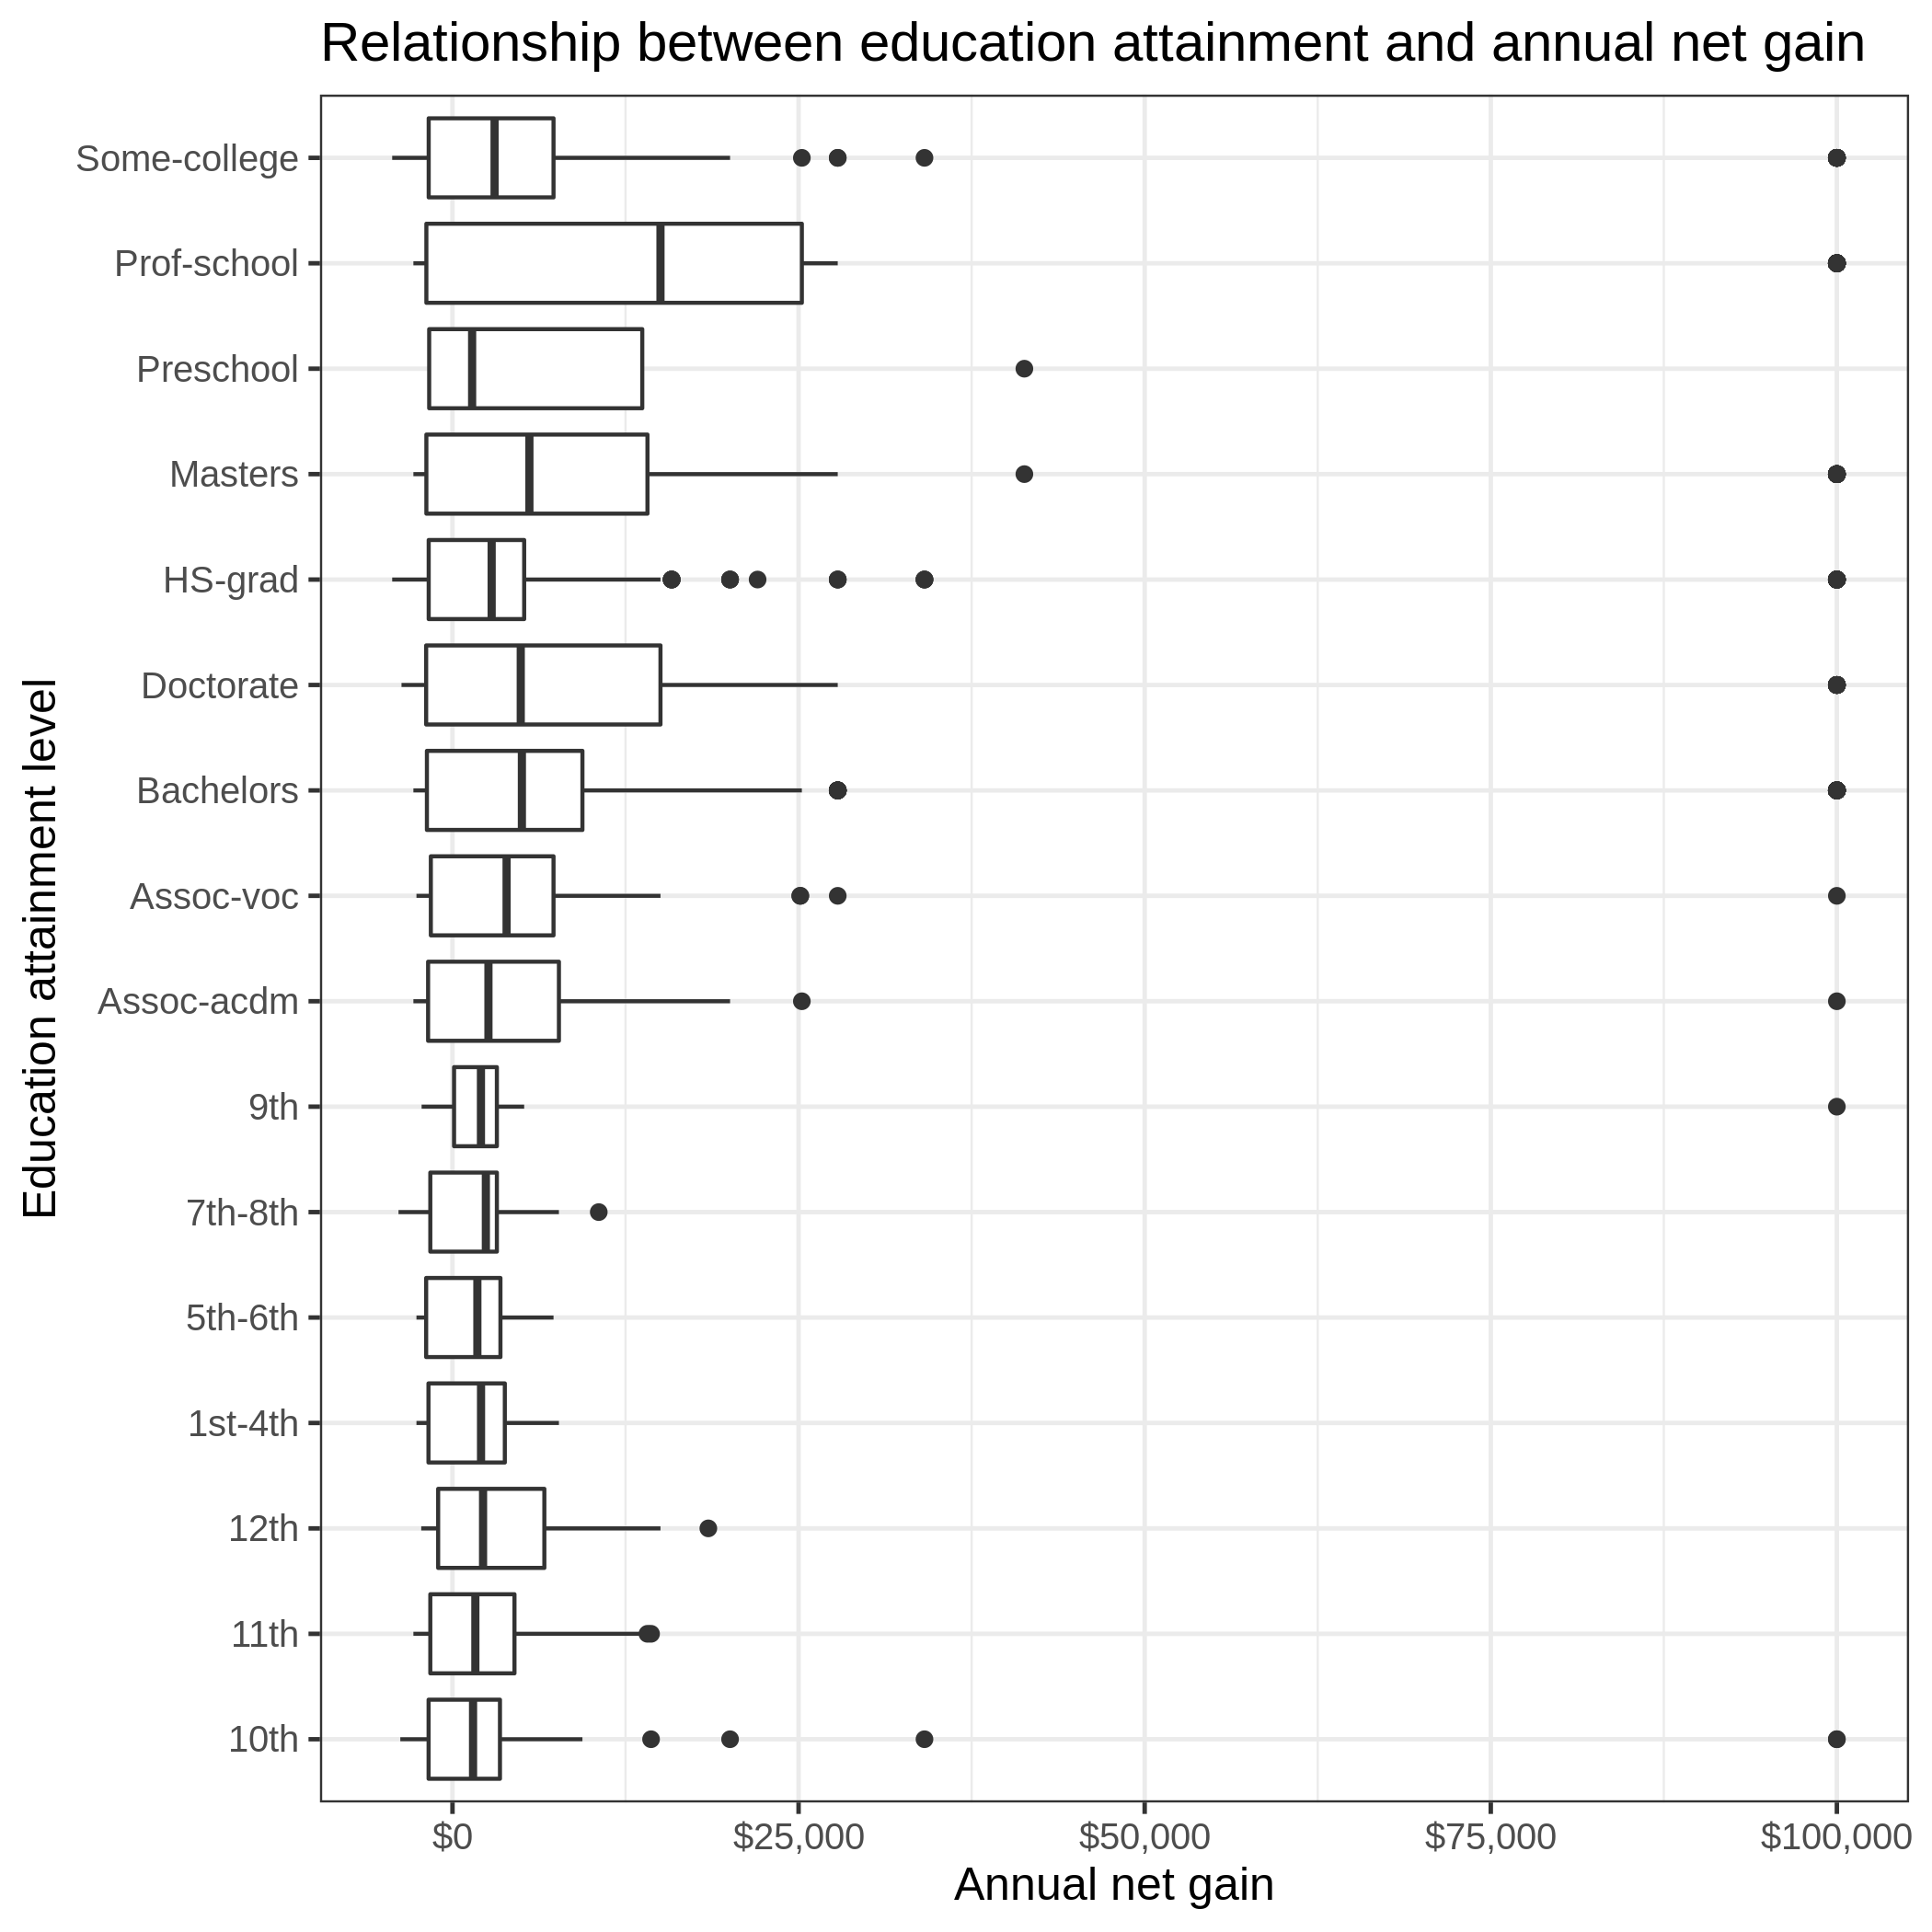
\includegraphics[width=0.75\linewidth]{/mnt/HDD/Documents/R_Projects/R Projects/group_08_ADULT-INCOME-1/images/net_education_plot} 

}

\caption{Figure 1: Boxplot of annual net capital gain across education levels}\label{fig:net-gain-education}
\end{figure}

Figure 1 shows that minimal correlation between annual net gain and
education attainment. However, there appeared to be a greater spread in
annual net gain for individuals with at least a high school diploma, and
persons with professional school education demonstrated the highest
median in annual net gain.

\hypertarget{eda-relationship-between-race-gender-and-annual-net-gain}{%
\subsubsection{EDA: Relationship between race, gender and annual net
gain}\label{eda-relationship-between-race-gender-and-annual-net-gain}}

We were interested to see if there were any visible patterns between
annual net gain and individucal's race and or gender. In the inital
exploratory data analysis, we examined the relationships between annual
net gain across race and gender.

\begin{Shaded}
\begin{Highlighting}[]
\NormalTok{knitr}\OperatorTok{::}\KeywordTok{include_graphics}\NormalTok{(}\KeywordTok{here}\NormalTok{(}\StringTok{"images/net_race_gender_plot.png"}\NormalTok{))}
\end{Highlighting}
\end{Shaded}

\begin{figure}

{\centering 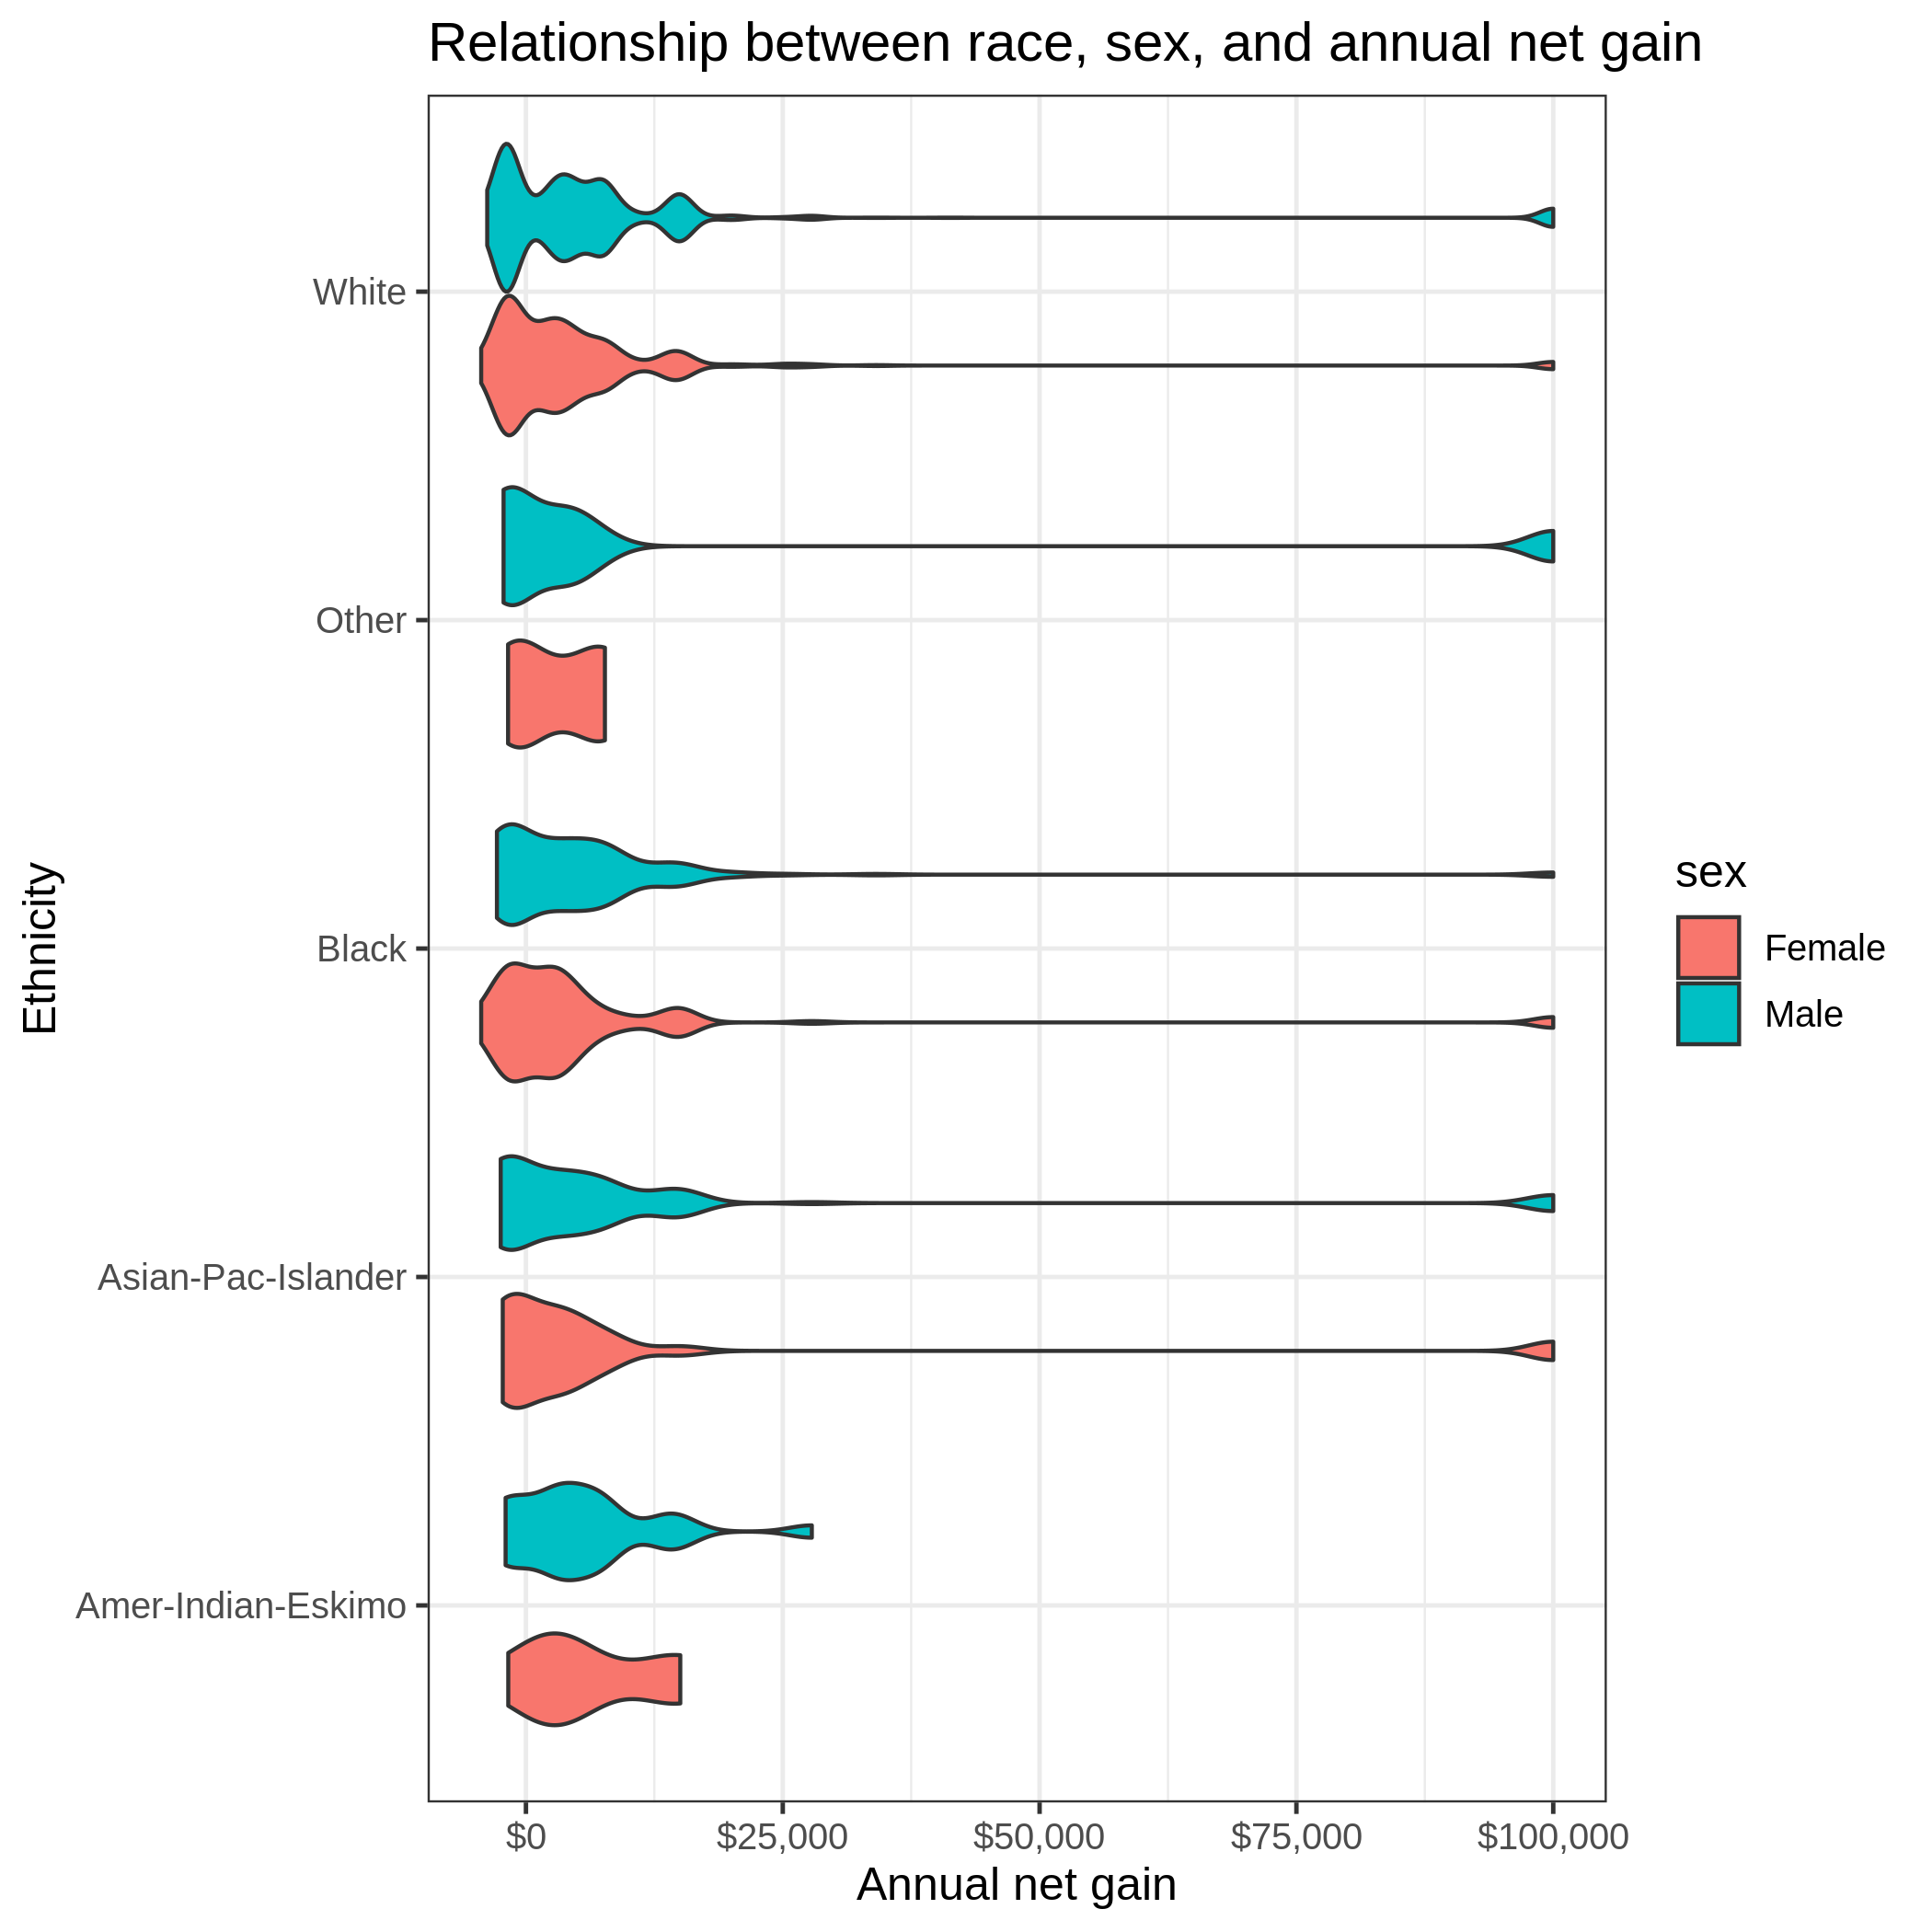
\includegraphics[width=0.75\linewidth]{/mnt/HDD/Documents/R_Projects/R Projects/group_08_ADULT-INCOME-1/images/net_race_gender_plot} 

}

\caption{Figure 2: Violin plot of annual net capital gain by ethnicity and sex}\label{fig:net-race-gender}
\end{figure}

There did not appear to be any significant differences in annual net
gain between sex across all ethnic groups (Figure 2). Moreover, no
obvious correlation between ethnicity and annual net gain was observed.

\hypertarget{eda-correlation-between-work-hours-per-week-and-annual-net-gain}{%
\subsubsection{EDA: Correlation between work hours per week and annual
net
gain}\label{eda-correlation-between-work-hours-per-week-and-annual-net-gain}}

We generated an additional script as part of the data analysis pipeline,
to plot the relationship between annual net gain and hours worked per
week. We categorized work hours per week as being short (under 25 hrs),
medium (25-50 hrs/wk), long (50-75 hrs/wk) and very long (over 75
hrs/wk).

\begin{figure}

{\centering 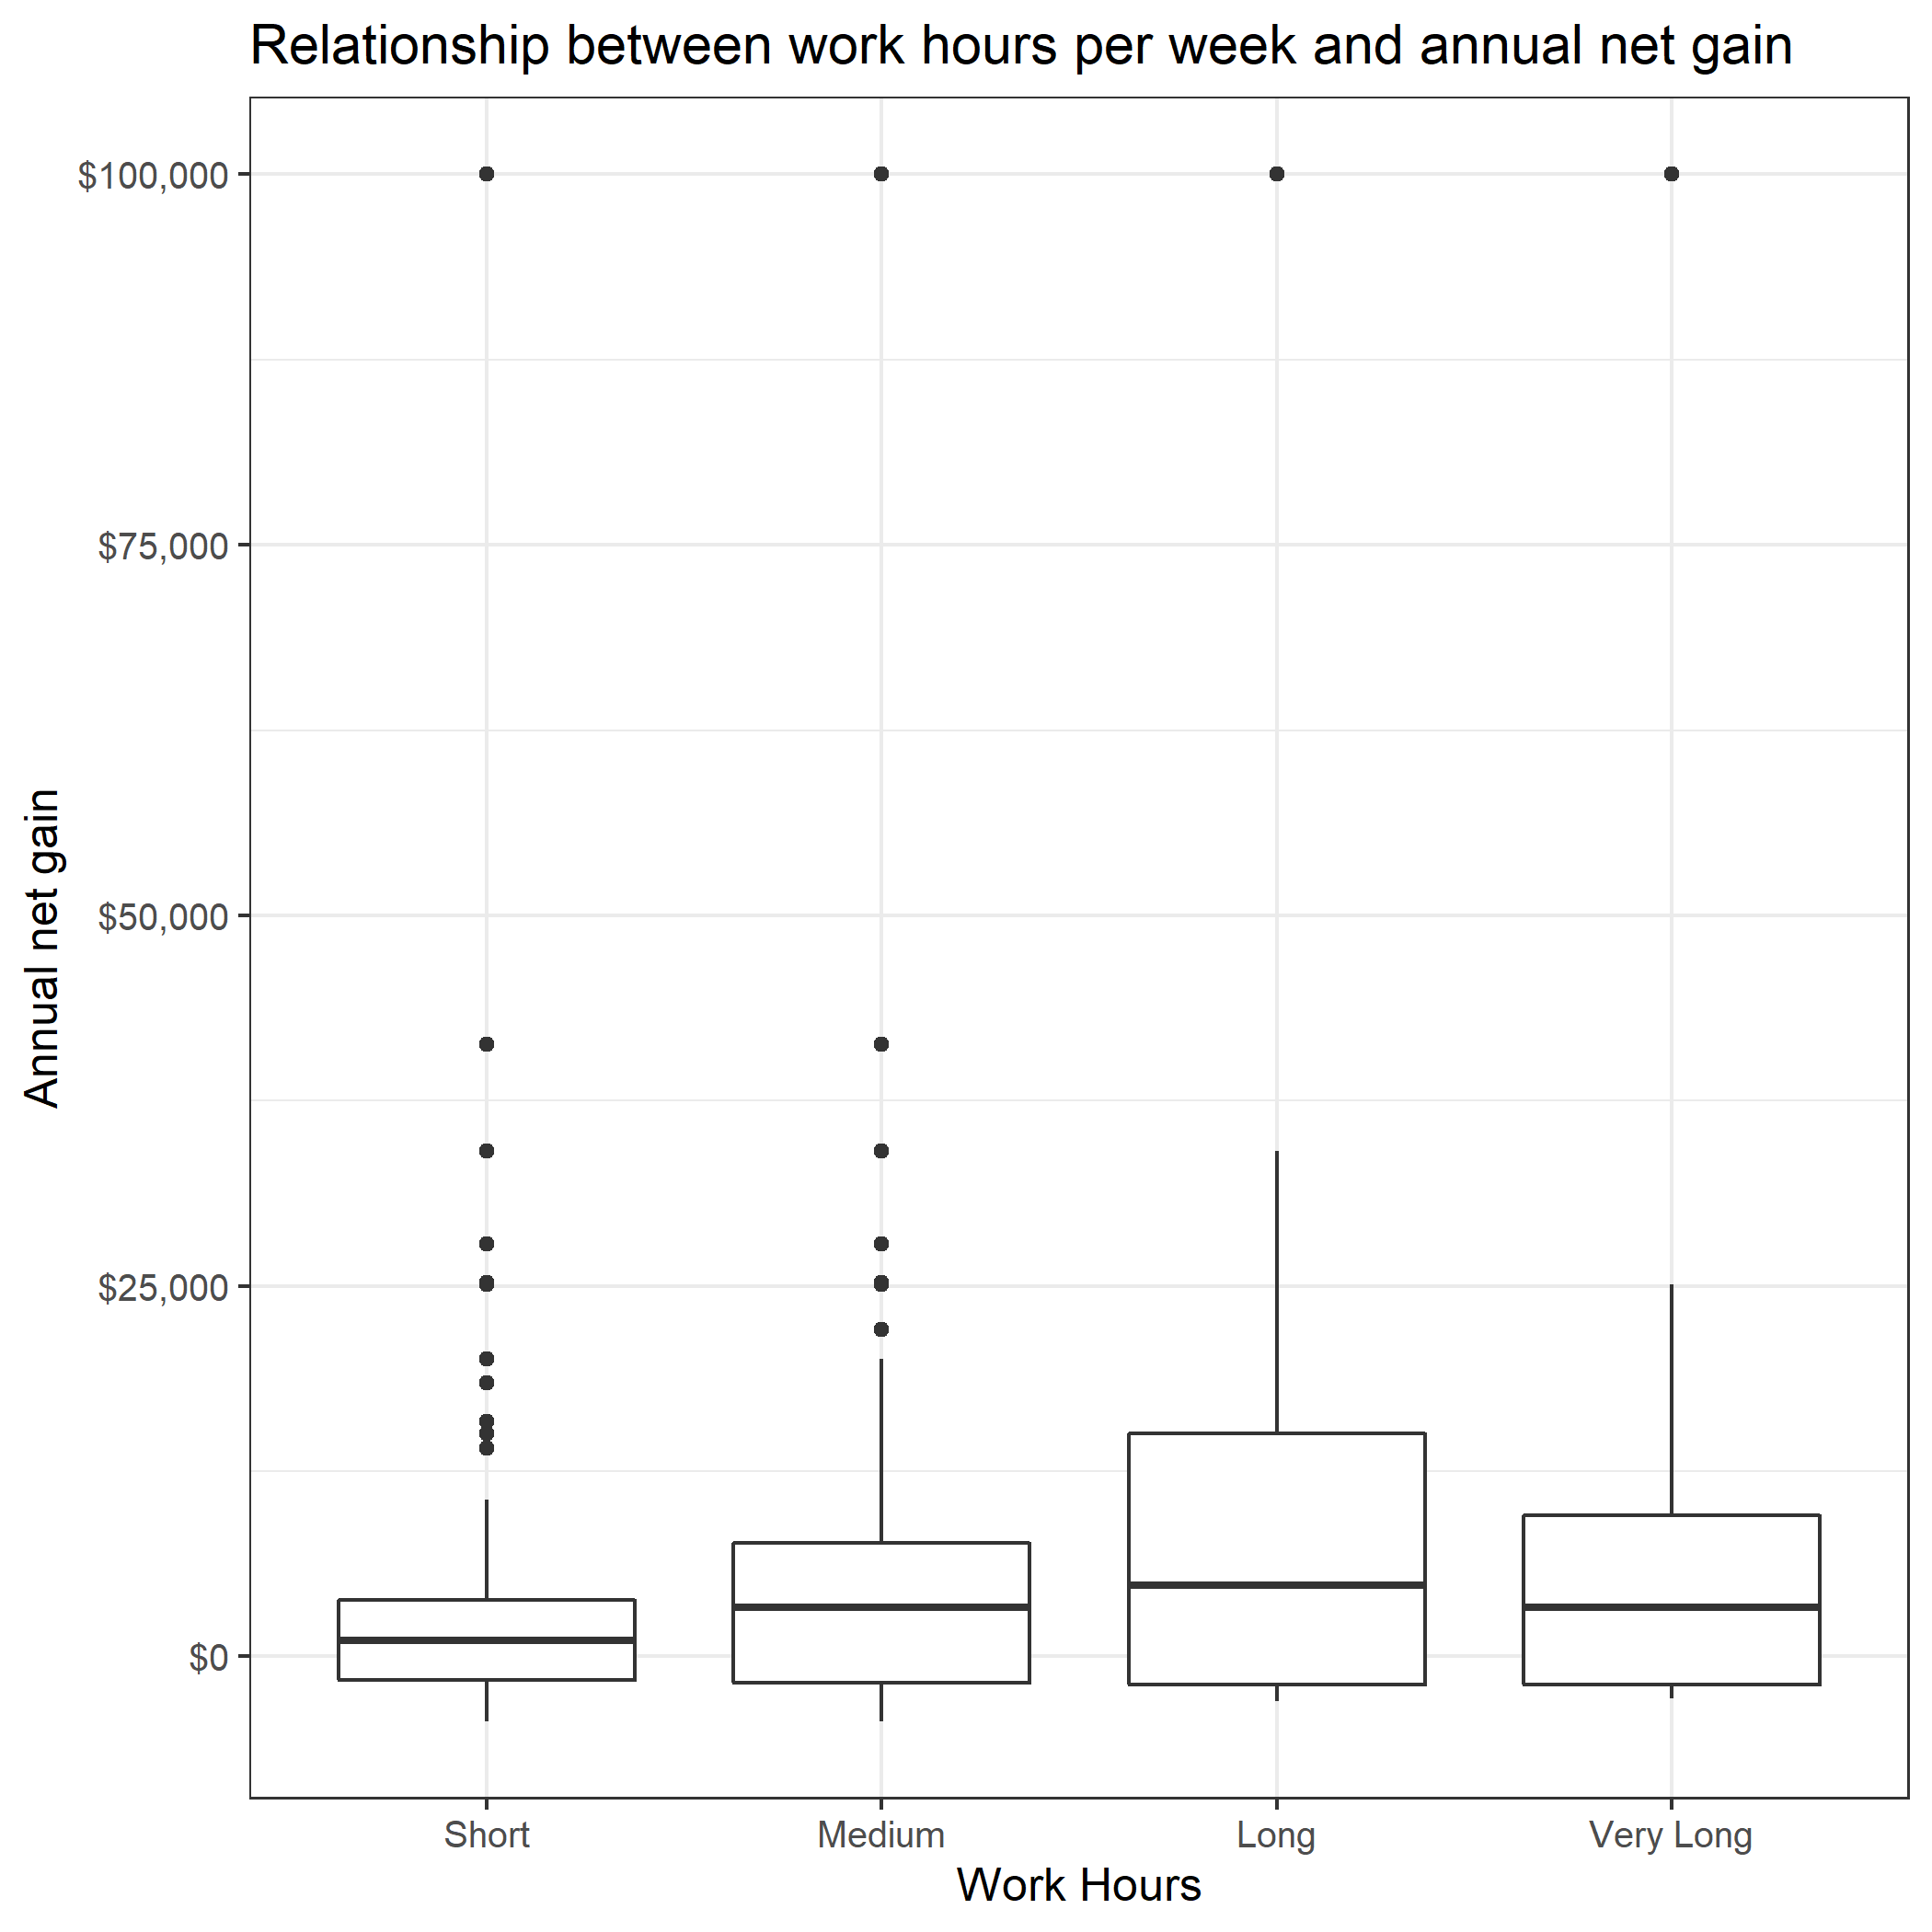
\includegraphics[width=0.75\linewidth]{/mnt/HDD/Documents/R_Projects/R Projects/group_08_ADULT-INCOME-1/images/net_work_hours_plot} 

}

\caption{Figure 3: Plot of annual net capital gain by hours worked per week}\label{fig:work-hours-plot}
\end{figure}

From the above boxplot, there appears to be an increase in annual net
gain from short to long work hours. However, the differences may not be
significant because greater variance in annual net gain is observed for
individuals with long work hours.

\hypertarget{linear-regression}{%
\subsection{Linear Regression}\label{linear-regression}}

A goal of this project was to generate a linear model for later use. The
`adult income' dataset did not have many linear relationships, so we
isolated a section of data which showed a more direct relationship
between variables in order to accomplish the scripting task of creating
a linear model. Figure 4 shows scatter plots of the relationship between
hours worked per week and age of worker, including the full dataset and
a subsection with a near-linear trend.

\begin{Shaded}
\begin{Highlighting}[]
\NormalTok{p1 <-}\StringTok{ }\NormalTok{dat }\OperatorTok\StringTok{ }
\StringTok{  }\KeywordTok{ggplot}\NormalTok{(}\KeywordTok{aes}\NormalTok{(}\DataTypeTok{x =}\NormalTok{ age, }\DataTypeTok{y =}\NormalTok{ hours_per_week))}\OperatorTok{+}
\StringTok{  }\KeywordTok{geom_jitter}\NormalTok{(}\DataTypeTok{alpha =} \FloatTok{0.4}\NormalTok{)}\OperatorTok{+}
\StringTok{  }\KeywordTok{theme_bw}\NormalTok{()}\OperatorTok{+}
\StringTok{  }\KeywordTok{labs}\NormalTok{(}\DataTypeTok{y =} \StringTok{"hrs/wk"}\NormalTok{, }\DataTypeTok{x =} \StringTok{""}\NormalTok{)}

\NormalTok{p2 <-}\StringTok{ }\NormalTok{dat }\OperatorTok\StringTok{ }
\StringTok{  }\KeywordTok{filter}\NormalTok{(age }\OperatorTok{<}\StringTok{ }\DecValTok{30}\NormalTok{,}
\NormalTok{         hours_per_week }\OperatorTok{!=}\StringTok{ }\DecValTok{40}\NormalTok{, hours_per_week }\OperatorTok{>=}\StringTok{ }\DecValTok{10}\NormalTok{) }\OperatorTok\StringTok{ }
\StringTok{  }\KeywordTok{ggplot}\NormalTok{(}\KeywordTok{aes}\NormalTok{(}\DataTypeTok{x =}\NormalTok{ age, }\DataTypeTok{y =}\NormalTok{ hours_per_week))}\OperatorTok{+}
\StringTok{  }\KeywordTok{geom_jitter}\NormalTok{(}\DataTypeTok{alpha =} \FloatTok{0.4}\NormalTok{)}\OperatorTok{+}
\StringTok{  }\KeywordTok{geom_smooth}\NormalTok{(}\DataTypeTok{method =}\NormalTok{ lm)}\OperatorTok{+}
\StringTok{  }\KeywordTok{labs}\NormalTok{(}\DataTypeTok{y =} \StringTok{"hrs/wk"}\NormalTok{, }\DataTypeTok{x =} \StringTok{"age of worker"}\NormalTok{)}\OperatorTok{+}
\StringTok{  }\NormalTok{ggpmisc}\OperatorTok{::}\KeywordTok{stat_poly_eq}\NormalTok{(}\DataTypeTok{formula =}\NormalTok{ y }\OperatorTok{~}\StringTok{ }\NormalTok{x, }
               \KeywordTok{aes}\NormalTok{(}\DataTypeTok{label =} \KeywordTok{paste}\NormalTok{(..eq.label.., ..rr.label.., }\DataTypeTok{sep =} \StringTok{"~~~"}\NormalTok{)), }
               \DataTypeTok{parse =} \OtherTok{TRUE}\NormalTok{, }\DataTypeTok{rr.digits =} \DecValTok{3}\NormalTok{)}\OperatorTok{+}
\StringTok{  }\KeywordTok{theme_bw}\NormalTok{()}

\CommentTok{# arrange plots}
\NormalTok{cowplot}\OperatorTok{::}\KeywordTok{plot_grid}\NormalTok{(p1, p2, }\DataTypeTok{align =} \StringTok{"v"}\NormalTok{, }\DataTypeTok{nrow =} \DecValTok{2}\NormalTok{,}
                   \DataTypeTok{labels =} \KeywordTok{c}\NormalTok{(}\StringTok{"A"}\NormalTok{, }\StringTok{"B"}\NormalTok{))}
\end{Highlighting}
\end{Shaded}

\begin{figure}

{\centering 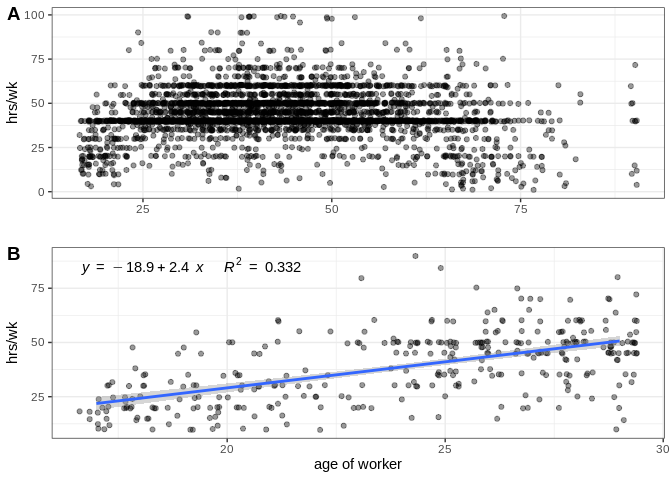
\includegraphics[width=0.75\linewidth]{FinalReport_milestone03_files/figure-latex/age-hours-1} 

}

\caption{Figure 4: Hours worked per week by age where plot 'A' shows the full dataset and plot 'B' shows a more linear section of filtered data (for workers under 30)}\label{fig:age-hours}
\end{figure}

The relationship between age and hours worked appeared to be loosely
parabolic. Work hours increased with age until approximately age 30-50,
at which time work hours stabilize before beginning to decrease with age
up to approximately 80 years old (Figure 4-A). In order to perform a
linear regression, we isolated the earlier part of this data, for
workers under the age of 30 who worked more than 10 hours per week and
not standard full time of 40 hours per week (Figure 4-B).

We wrote a script to generate a linear model based on the filtered data
shown in Figure 4-B, as well as a script to generate that sub-plot as a
stand-alone graphic.

\begin{figure}

{\centering 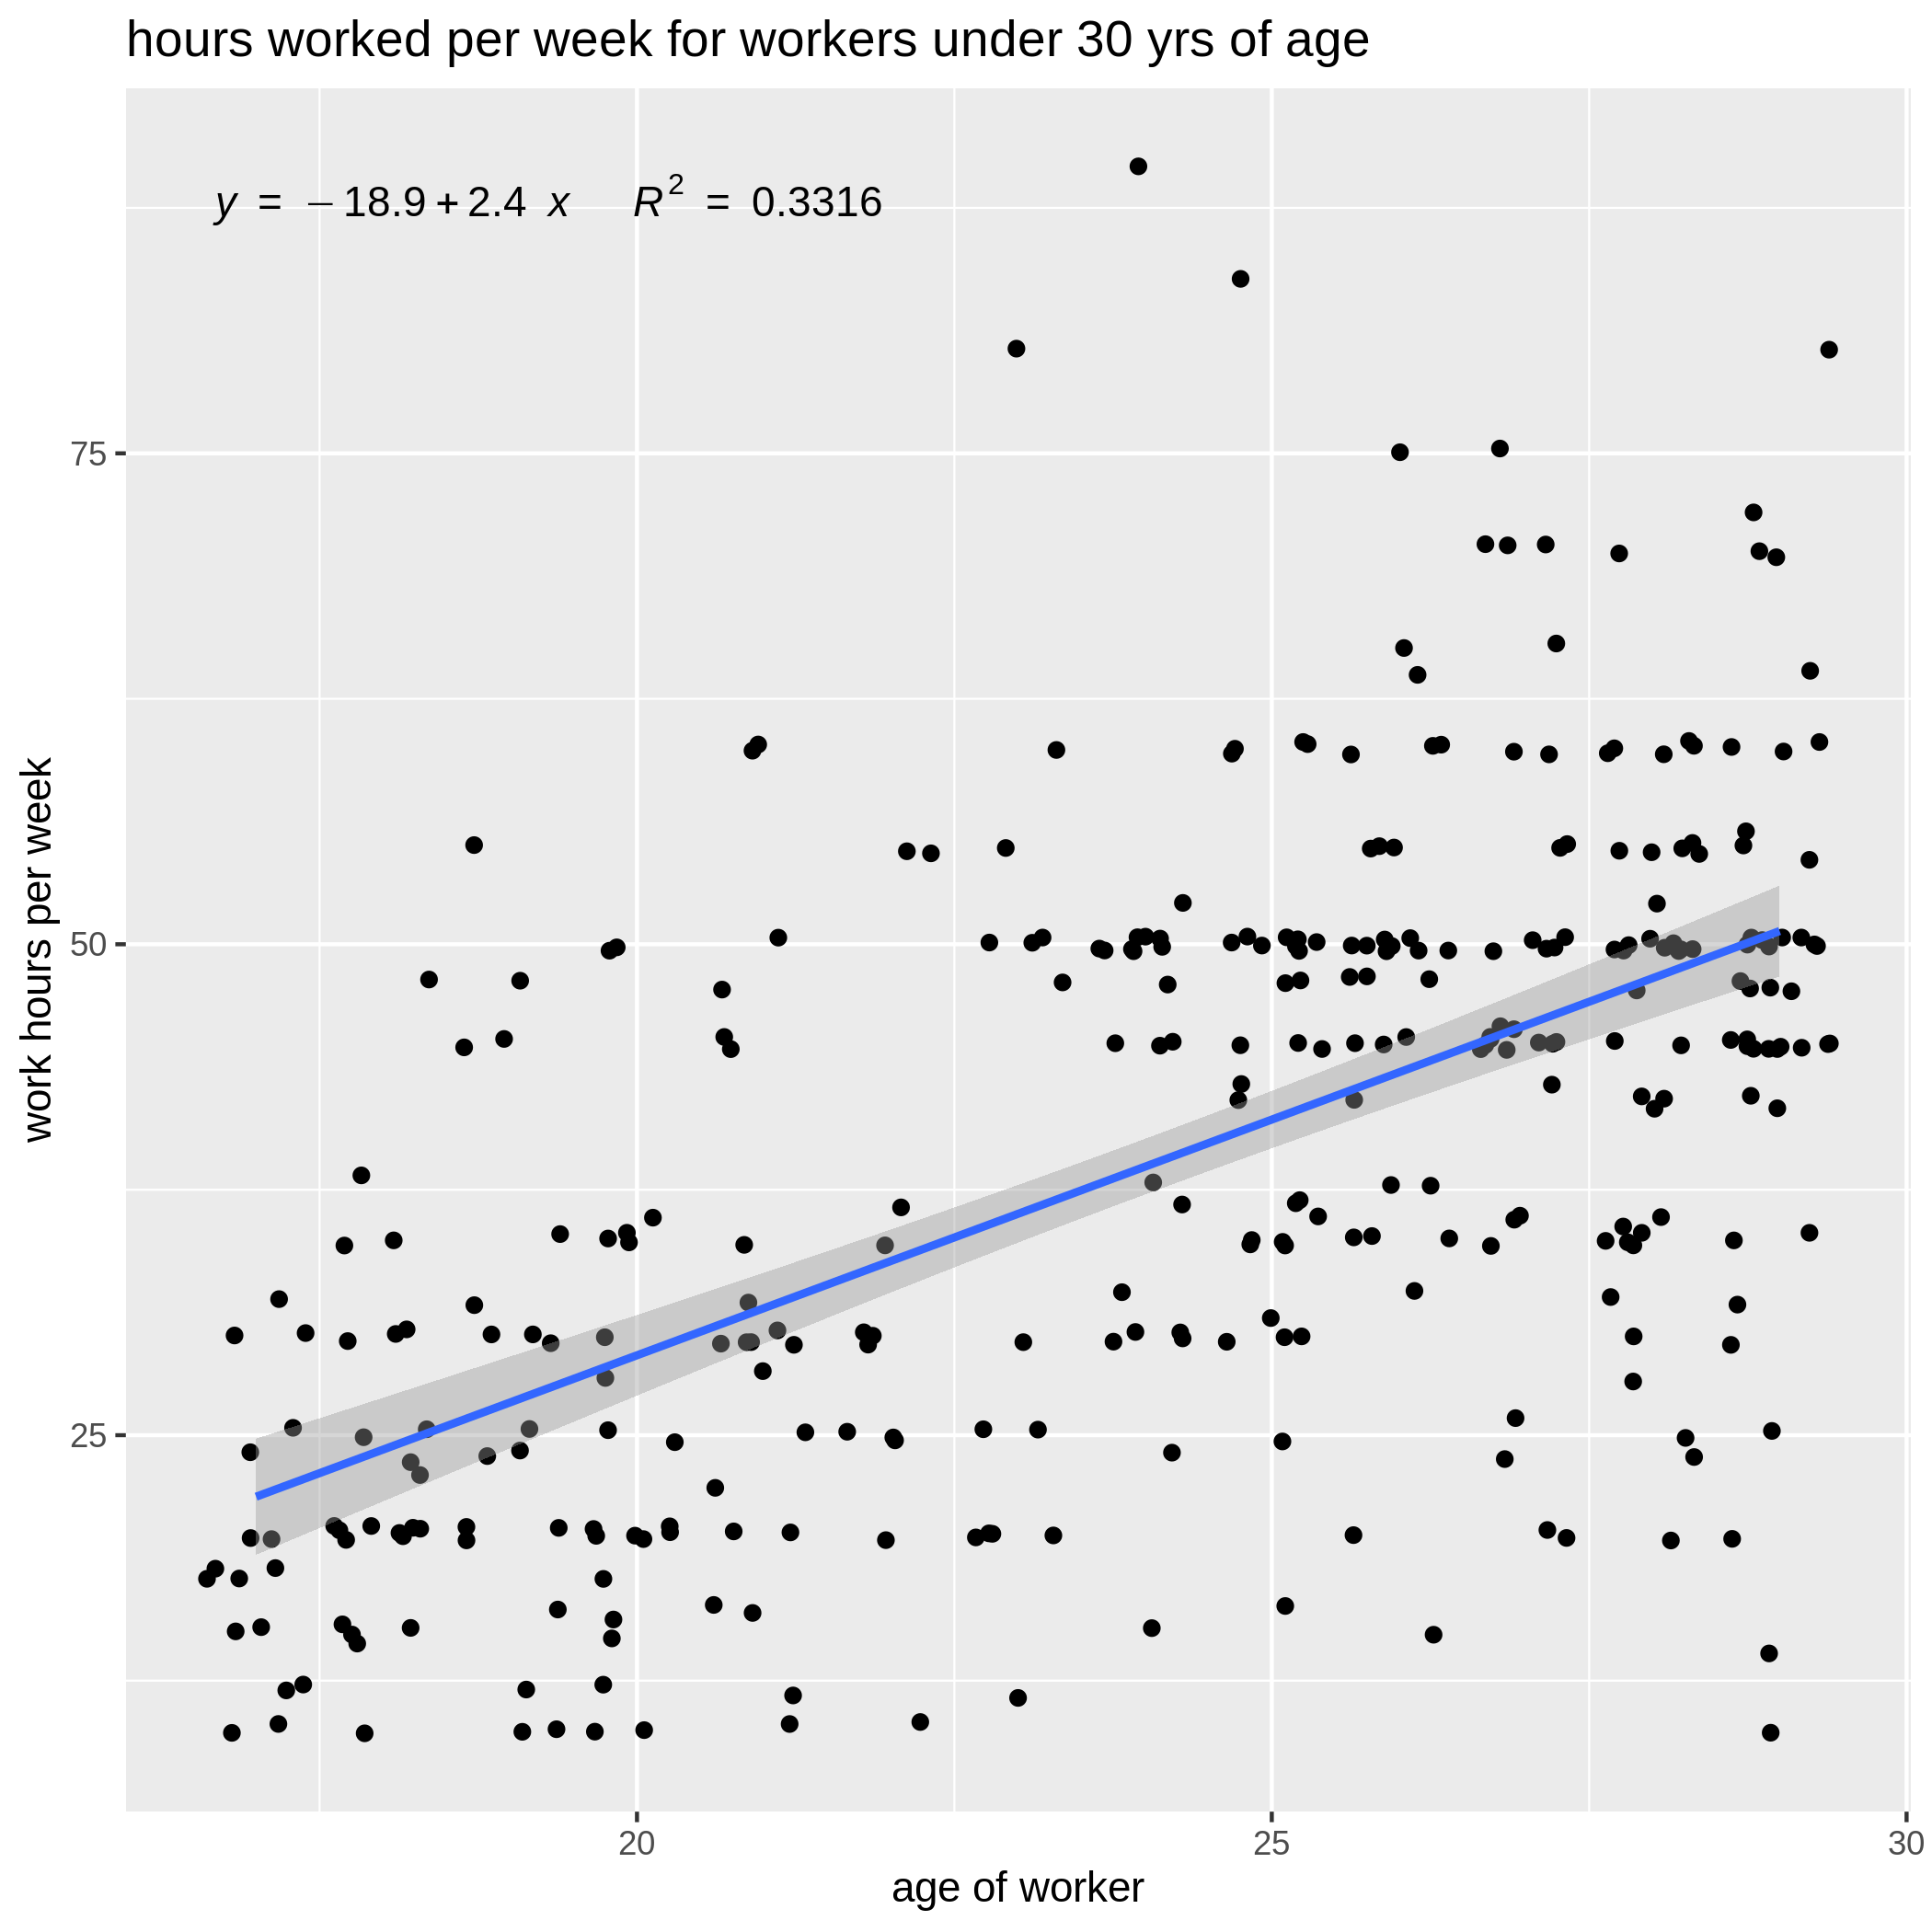
\includegraphics[width=0.75\linewidth]{/mnt/HDD/Documents/R_Projects/R Projects/group_08_ADULT-INCOME-1/images/linear-regression_plot} 

}

\caption{Figure 5: Plot of linear regression model data for hours worked by those under age 30}\label{fig:age-hrs-plot}
\end{figure}

\hypertarget{references}{%
\subsection{References}\label{references}}

United States Census Bureau, 2016. Income and Poverty, `about income'.
\url{https://www.census.gov/topics/income-poverty/income/about.html}

University of California Irvine, Machine Learning Repository.
\url{https://archive.ics.uci.edu/ml/datasets/adult}.

\end{document}
